\documentclass[margin=1mm]{standalone}
\usepackage[utf8]{inputenc}
\usepackage{amsmath}
\usepackage{amsfonts}
\usepackage{amssymb, bm}
\usepackage{tikz}
\usetikzlibrary{calc,arrows,positioning,shapes,shapes.gates.logic.US,trees, backgrounds}
\usetikzlibrary{decorations.pathreplacing}
\usetikzlibrary{fit, positioning}

\begin{document}
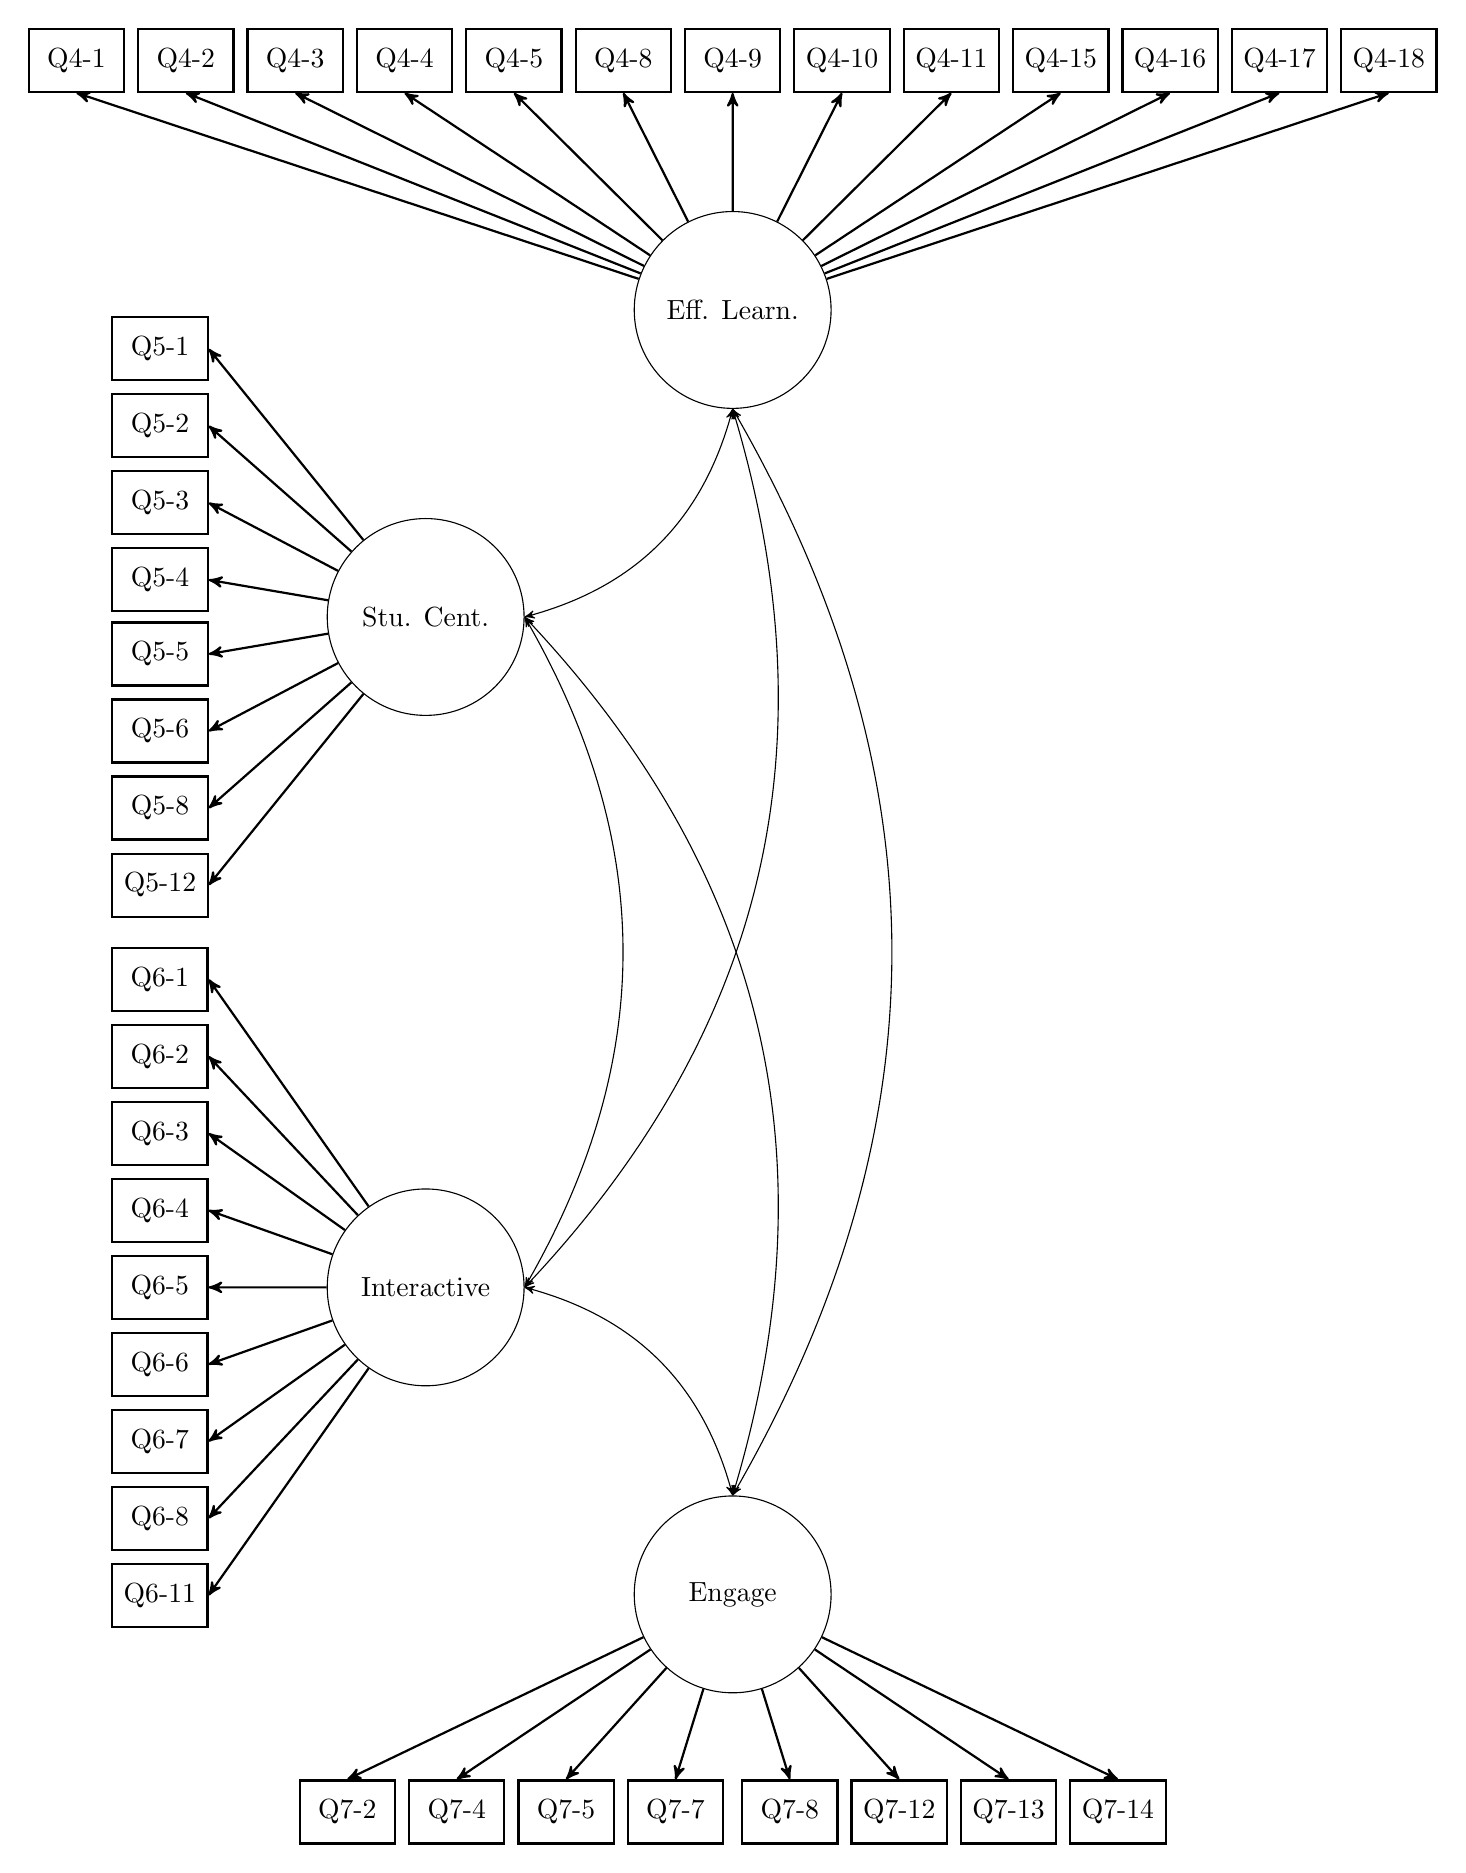
\begin{tikzpicture}[auto,scale=3,
	latent/.style={circle,draw,text badly centered, inner sep=2pt,minimum size=25mm},
	error/.style={circle,draw,text badly centered, inner sep=2pt,minimum size=10mm},
	manifest/.style={text centered, rectangle,draw,thick,inner sep=3pt,minimum height=8mm, minimum width=10mm, text width= 10mm},
	  plate/.style={draw, shape=rectangle,thick, minimum height=4.25cm, minimum width=4.5cm, text width=1cm, align=right, inner sep=10pt, inner ysep=10pt, append after command={node[below right= 3pt of \tikzlastnode.north west] {#1}}},
	  plate2/.style={draw, shape=rectangle,thick, minimum height=4.5cm, minimum width=7cm, text width=1cm, align=right, inner sep=5pt, inner ysep=8pt, append after command={node[left= 3pt of \tikzlastnode.east] {#1}}},
	manifestRot/.style={text centered, rectangle, draw, thick,inner sep=3pt, minimum width=7mm, text width= 7mm, minimum height=15},
	manifestfront/.style={rectangle,draw,thick,inner sep=0pt,minimum size=12mm, fill=white},
	ghost/.style={rectangle, inner sep=0pt,text centered,    minimum height=0mm, minimum width=5mm, text width= 5 mm},
	lcorr/.style={<->,>=stealth', bend right=40},
	rcorr/.style={<->,>=stealth', bend left=40},
	fcorr/.style={<->,>=stealth', bend left=40},
	ofcorr/.style={<->,>=stealth', bend right=30},
	ofcorr2/.style={<->,>=stealth', bend left=30},
	intercept/.style={regular polygon,
        regular polygon sides=3,draw,thick,inner sep=0pt,minimum size=10mm},
	mean/.style={regular polygon,regular polygon sides=3,draw,thick,inner sep=0pt,minimum size=10mm},
	paths/.style={->, thick, >=stealth'},
	variance/.style={<->, thick, >=stealth', bend left=270, looseness=2},
	varianceTop/.style={<->, thick, >=stealth', bend right=270, looseness=2},
	unique/.style={<->, thick, >=stealth', loop below=270, looseness=8},
	factvar/.style={<->, thick, >=stealth', loop right=270, looseness=8}
	] % End Creating Path Model Pieces
\tikzset{mystyle/.style={->,double=black}}


% Student Centered
\node [latent] at (0,0) (sc) {Stu. Cent.};
\node [ghost] [left= 1.86cm of sc] (g1) {};
\node [manifest] [above = 0.05cm of g1] (q54) {Q5-4};
\node [manifest] [above = 0.15cm of q54] (q53) {Q5-3};
\node [manifest] [above = 0.15cm of q53] (q52) {Q5-2};
\node [manifest] [above = 0.15cm of q52] (q51) {Q5-1};
\node [manifest] [below = 0.05cm of g1] (q55) {Q5-5};
\node [manifest] [below = 0.15cm of q55] (q56) {Q5-6};
\node [manifest] [below = 0.15cm of q56] (q58) {Q5-8};
\node [manifest] [below = 0.15cm of q58] (q512) {Q5-12};

% Effective Learning
\node [latent] [above right = 3cm of sc] (el) {Eff. Learn.};
\node [manifest] [above = 1.5cm of el] (q49) {Q4-9};
\node [manifest] [left = 0.15cm of q49] (q48) {Q4-8};
\node [manifest] [left = 0.15cm of q48] (q45) {Q4-5};
\node [manifest] [left = 0.15cm of q45] (q44) {Q4-4};
\node [manifest] [left = 0.15cm of q44] (q43) {Q4-3};
\node [manifest] [left = 0.15cm of q43] (q42) {Q4-2};
\node [manifest] [left = 0.15cm of q42] (q41) {Q4-1};
\node [manifest] [right = 0.15cm of q49] (q410) {Q4-10};
\node [manifest] [right = 0.15cm of q410] (q411) {Q4-11};
\node [manifest] [right = 0.15cm of q411] (q415) {Q4-15};
\node [manifest] [right = 0.15cm of q415] (q416) {Q4-16};
\node [manifest] [right = 0.15cm of q416] (q417) {Q4-17};
\node [manifest] [right = 0.15cm of q417] (q418) {Q4-18};


% Interactive
\node [latent] [below = 6cm of sc] (in) {Interactive};
\node [manifest] [left = 1.5cm of in] (q65) {Q6-5};
\node [manifest] [above = 0.15cm of q65] (q64) {Q6-4};
\node [manifest] [above = 0.15cm of q64] (q63) {Q6-3};
\node [manifest] [above = 0.15cm of q63] (q62) {Q6-2};
\node [manifest] [above = 0.15cm of q62] (q61) {Q6-1};
\node [manifest] [below= 0.15cm of q65] (q66) {Q6-6};
\node [manifest] [below= 0.15cm of q66] (q67) {Q6-7};
\node [manifest] [below= 0.15cm of q67] (q68) {Q6-8};
\node [manifest] [below= 0.15cm of q68] (q611) {Q6-11};

% Engagedness
\node [latent] [below right = 3cm of in] (en) {Engage};
\node [ghost] [below = 1.5cm of en] (g2) {};
\node [manifest] [left = -0.15cm of g2] (q77) {Q7-7};
\node [manifest] [left = 0.15cm of q77] (q75) {Q7-5};
\node [manifest] [left = 0.15cm of q75] (q74) {Q7-4};
\node [manifest] [left = 0.15cm of q74] (q72) {Q7-2};
\node [manifest] [right = -0.15cm of g2] (q78) {Q7-8};
\node [manifest] [right = 0.15cm of q78] (q712) {Q7-12};
\node [manifest] [right = 0.15cm of q712] (q713) {Q7-13};
\node [manifest] [right = 0.15cm of q713] (q714) {Q7-14};


% paths
\draw[paths] (el)  -- (q41.south);
\draw[paths] (el)  -- (q42.south);
\draw[paths] (el)  -- (q43.south);
\draw[paths] (el)  -- (q44.south);
\draw[paths] (el)  -- (q45.south);
\draw[paths] (el)  -- (q48.south);
\draw[paths] (el)  -- (q49.south);
\draw[paths] (el)  -- (q410.south);
\draw[paths] (el)  -- (q411.south);
\draw[paths] (el)  -- (q415.south);
\draw[paths] (el)  -- (q416.south);
\draw[paths] (el)  -- (q417.south);
\draw[paths] (el)  -- (q418.south);

\draw[paths] (sc)  -- (q51.east);
\draw[paths] (sc)  -- (q52.east);
\draw[paths] (sc)  -- (q53.east);
\draw[paths] (sc)  -- (q54.east);
\draw[paths] (sc)  -- (q55.east);
\draw[paths] (sc)  -- (q56.east);
\draw[paths] (sc)  -- (q58.east);
\draw[paths] (sc)  -- (q512.east);

\draw[paths] (in)  -- (q61.east);
\draw[paths] (in)  -- (q62.east);
\draw[paths] (in)  -- (q63.east);
\draw[paths] (in)  -- (q64.east);
\draw[paths] (in)  -- (q65.east);
\draw[paths] (in)  -- (q66.east);
\draw[paths] (in)  -- (q67.east);
\draw[paths] (in)  -- (q68.east);
\draw[paths] (in)  -- (q611.east);

\draw[paths] (en)  -- (q72.north);
\draw[paths] (en)  -- (q74.north);
\draw[paths] (en)  -- (q75.north);
\draw[paths] (en)  -- (q77.north);
\draw[paths] (en)  -- (q78.north);
\draw[paths] (en)  -- (q712.north);
\draw[paths] (en)  -- (q713.north);
\draw[paths] (en)  -- (q714.north);

% factor covariances
\draw[ofcorr2] (el.south) to (sc.east);
\draw[ofcorr2] (el.south) to (in.east);
\draw[ofcorr2] (el.south) to (en.north);
\draw[ofcorr2] (sc.east) to (in.east);
\draw[ofcorr2] (sc.east) to (en.north);
\draw[ofcorr2] (in.east) to (en.north);


\end{tikzpicture}
\end{document}